\section{Settings}

The customization (settings) of the game is linked to requirements \ref{sprint2:requirements:profile}, \ref{sprint2:requirements:calibrate}, \ref{sprint2:tab1:req10}, \ref{sprint2:requirements:avoidorpickup}, and \ref{sprint2:requirements:categorymode} (see \cref{sprint2:requirement_table_1}).

\paragraph{Note:} Requirements \ref{sprint2:tab1:req11} and \ref{sprint2:tab1:req12} are also linked to settings, but this is handled seperately by the ''map editor'', which is explained in \cref{sprint2:map_editor}.\\

\noindent
The settings activity handles three things; Altering the speed of the car, Changing the colors of the garages, and Calibrating the microphone.
A screenshot of the settings activity can be seen in \cref{sprint2:settings:fig}.

\begin{center}
\begin{figure}
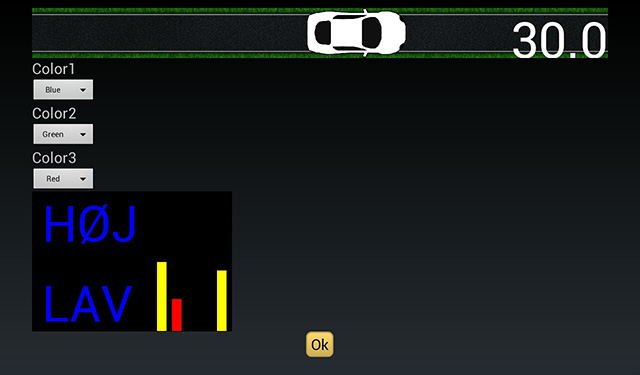
\includegraphics[width=\textwidth]{settings}
\caption{The settings activity}
\label{sprint2:settings:fig}
\end{figure}
\end{center}

\paragraph{Speed} is changed by tapping the ends of a small fragment of the game, displaying only one lane and the moving car.
By tapping the left end, the speed is decreased and by tapping the right, it is increased.
Whenever a change to speed is made, it is immediately visible in the game fragment.

\paragraph{Color} is as of now changed by picking a color from a dropdown box.
\mikael{This however is supposed to be a color picker, but it was at creation time not in the graphics components library (giraf-components).}

\paragraph{Microphone Calibration} is done in a small game fragment, as can be seen in the bottom of the settings screenshot.
The way it is done atm, is when holding either 'H\o j' (high) or 'Lav' (low) down, during this time the microphone records and when they are released the average of all the recordings during the time are averaged and set as the appropriate threshold value.
\mikael{This does not work well. Also, the fragment was supposed to show the car moving up and down, so that the current calibration and its effect on the car could be seen.}